\documentclass[twocolumn]{IEEEtran}

\usepackage[ansinew]{inputenc} 
\usepackage{amsmath}
\usepackage{graphicx}
\usepackage{graphics}
\usepackage{hyperref}
\usepackage{longtable}               
\usepackage{fancyhdr}
\usepackage{times}
\usepackage{color}                   
\usepackage{makeidx}                 
\usepackage{cite}
\usepackage{float}
\setcounter{page}{1}

\usepackage{listings}
\usepackage{color}

\definecolor{mygreen}{rgb}{0,0.6,0}
\definecolor{mygray}{rgb}{0.5,0.5,0.5}
\definecolor{mymauve}{rgb}{0.58,0,0.82}
\lstset{ %
  backgroundcolor=\color{white},   % choose the background color; you must add \usepackage{color} or \usepackage{xcolor}
  basicstyle=\footnotesize,        % the size of the fonts that are used for the code
  breakatwhitespace=false,         % sets if automatic breaks should only happen at whitespace
  breaklines=true,                 % sets automatic line breaking
  captionpos=b,                    % sets the caption-position to bottom
  commentstyle=\color{mygreen},    % comment style
  deletekeywords={...},            % if you want to delete keywords from the given language
  escapeinside={\%*}{*)},          % if you want to add LaTeX within your code
  extendedchars=true,              % lets you use non-ASCII characters; for 8-bits encodings only, does not work with UTF-8
  frame=single,                    % adds a frame around the code
  keepspaces=true,                 % keeps spaces in text, useful for keeping indentation of code (possibly needs columns=flexible)
  keywordstyle=\color{blue},       % keyword style
  language=Matlab,                 % the language of the code
  morekeywords={*,...},            % if you want to add more keywords to the set
  numbers=left,                    % where to put the line-numbers; possible values are (none, left, right)
  numbersep=5pt,                   % how far the line-numbers are from the code
  numberstyle=\tiny\color{mygray}, % the style that is used for the line-numbers
  rulecolor=\color{white},         % if not set, the frame-color may be changed on line-breaks within not-black text (e.g. comments (green here))
  showspaces=false,                % show spaces everywhere adding particular underscores; it overrides 'showstringspaces'
  showstringspaces=false,          % underline spaces within strings only
  showtabs=false,                  % show tabs within strings adding particular underscores
  stepnumber=2,                    % the step between two line-numbers. If it's 1, each line will be numbered
  stringstyle=\color{mymauve},     % string literal style
  tabsize=2,                       % sets default tabsize to 2 spaces
  title=\lstname                   % show the filename of files included with \lstinputlisting; also try caption instead of title
}


\begin{document}
\include{./imagenes}

\title{Identificaci�n de una planta de 3 Opams (sistema de tercer orden) utilizando la estructura param�trica ARMAX.}


\author{Autores \\ 
				Estrada Vidal, Jorge  \textcolor{blue}{jor1550g@gmail.com} \\
				Florian Chacon, Erick  \textcolor{blue}{erick.florian.uni@gmail.com} \\
				Giraldo Castillo, Oscar \textcolor{blue}{oscar.gi.cast@gmail.com} \\ 		
				\vspace{4 mm}
				Asesores: \\
				Ing. Rodriguez Bustinza, Ricardo \textcolor{blue}{robust@uni.edu.pe} \\ 	
				
				\vspace{8 mm}
				\emph{Universidad Nacional de Ingenier\'ia}
		}			

		
		
%\markboth{IEEE Trans...}{Murray and Balemi: ...}
\maketitle





\section{OBJETIVOS} %%%%%%%%%%%%%%%%%%%%%%%%%%%%%%%%%%%%%%%%%%%%%%%%%%%%%%%%%%%%%%%%%%%%%%%%%%%%%%%%%%%%%%%%%%%%%%%%%%%%%%%%%

\begin{itemize} \item Identificar el modelo de un planta de 3 Op-Amp?s a trav�s de la adquisici�n de datos y de la estructura param�trica ARMAX \end{itemize}

\section{MARCO TE�RICO}%%%%%%%%%%%%%%%%%%%%%%%%%%%%%%%%%%%%%%%%%%%%%%%%%%%%%%%%%%%%%%%%%%%%%%%%%%%%%%%

% ----------------------------------------------------------------------------------------------------
\subsection{Estructuras de modelos parametricos}
Las estructuras de modelos tambien conocidas como ``cajas negras'' quedan representadas por ejemplo, mediante una ecuaci�n lineal en diferencias dado por:

% ------------ Ecuacion numero 1 --------------
\begin{eqnarray}
\nonumber y \big(t\big) + a_{1} y \big(t-1\big) +...+ a_{ n_{a} } y \big(t- n_{a} \big) = \\
b_{1}  u_{t-1} +...+ b_{ n_{b} } y \big(t- n_{b} \big) +e \big(t\big) \label{eq:1}
\end{eqnarray}
% -------------- FIN DE ECUACION --------------

El termino de ruido blanco, e(t) aca ingresa como un error directo en la ecuacion en diferencias dada en ~\ref{eq:1}, a menudo es llamada ecuacion del modelo de error (estructura).\\

El vector que es llamado vector de parametros es el objetivo del estudio, es decir, encontrando dicho vector podemos conocer el modelo discreto y por ende el modelo continuo.

% ------------ Ecuacion numero 2 --------------
\begin{eqnarray}
 \theta = \big(
 \begin{array}{ccccccc}
 a_{1} & a_{2} & \cdots &  a_{ n_{a} } & b_{1} & \cdots &  b_{ n_{b} }
\end{array}
\big)  ^{T} \label{eq:2}
\end{eqnarray}
% -------------- FIN DE ECUACION --------------

Dentro de estas estructuras parametricas principales que nos proporcionan las herramientas del software de simulacion de Matlab y LabVIEW est�:\\

\paragraph{Estructura Parametrica ARX}
\paragraph{Estructura Parametrica ARMAX}
\paragraph{Estructura Parametrica OE (Output Error)}
\paragraph{Estructura Parametrica BJ (Box Jenkins)}

En este laboratorio, estudiaremos la segunda estructura que describiremos a continuaci�n:

% ----------------------------------------------------------------------------------------------------
\subsection{Estructura ARMAX}
El modelo ARMAX (AutoRegresive eXogenous Moving Average) es mas flexible describiendo la ecuacion de error como un ``promedio movil'', el ruido blanco puede ser representado por e(t), el modelo presenta la relacion de entrada y salida que puede ser descrita por una ecuacion en diferencia lineal en la forma.

% ------------ Ecuacion numero 3 --------------
\begin{eqnarray}
y\big(t\big) = \frac{B \big(q\big) }{A \big(q\big) } U \big(t\big)+ \frac{C \big(q\big) }{A \big(q\big) } e \big(t\big) \label{eq:3}
\end{eqnarray}
% -------------- FIN DE ECUACION --------------

Siendo su funci�n de transferencia:

% ------------ Ecuacion numero 4 --------------
\begin{eqnarray}
Y\big(z\big) = \frac{B \big(z\big) }{A \big(z\big) }  z^{-d}U \big(z\big)+ \frac{C \big(z\big) }{A \big(z\big) } E \big(z\big) \label{eq:4}
\end{eqnarray}
% -------------- FIN DE ECUACION --------------

%\begin{figure}[h!]
%	\centering % Requires \usepackage{graphicx}
% 	\includegraphics[height=4cm]{images/ARMAX_structure.png}
% 	\caption{Estructura ARMAX.}
% 	\label{fig:armax_structure}
%\end{figure}

A continuaci�n presentamos un esquema b�sico del sistema analizado (ver Fig. ~\ref{fig:system_diagram}).\\

%\begin{figure}[h!]
%  \centering
%    \includegraphics[height=4cm]{images/system_diagram.png}
%  \caption{Esquema b�sico del sistema analizado}
%  \label{fig:system_diagram}
%\end{figure}

En donde el bloque etiquetado como planta contiene lo siguiente: (ver Fig. ~\ref{fig:system_proteus})

%\begin{figure}[h!]
%  \centering
%    \includegraphics[height=4cm]{images/system_proteus.png}
%  \caption{Esquema realizado en Proteus}
%  \label{fig:system_proteus}
%\end{figure}

Cuya simulaci�n obtenida en Proteus es la siguiente: (ver Fig. ~\ref{fig:simulation_proteus})

%\begin{figure}[h!]
%  \centering
%    \includegraphics[height=4cm]{images/simulation_proteus.png}
%  \caption{Respuesta de la planta a la funci�n Gate}
%  \label{fig:simulation_proteus}
%\end{figure}
 

\section{PRESENTACI�N DE RESULTADOS} %%%%%%%%%%%%%%%%%%%%%%%%%%%%%%%%%%%%%%%%%%%%%%%%%%%%%%%%%%%%%%%%%%%%%%%%%%%%%%%%%%%%%%%%%%%%%%%%%%%%%%%%%%

En este capitulo mostraremos los resultados del an�lisis anterior. LLegando a obtener:
\begin{itemize}
\item Dise�o anal�gico de un controlador PI.
\item Redise�o digital de un controlador PI por Tustin.
\item Comparaci�n entre control PI y PID.
\end{itemize}
 
\subsection{MATLAB}

La data obtenida de la adquisici�n se puede apreciar en la figura ~\ref{fig:data}
\begin{figure}[h!]
	\centering 
	\graphicspath{./imagenes/}
 	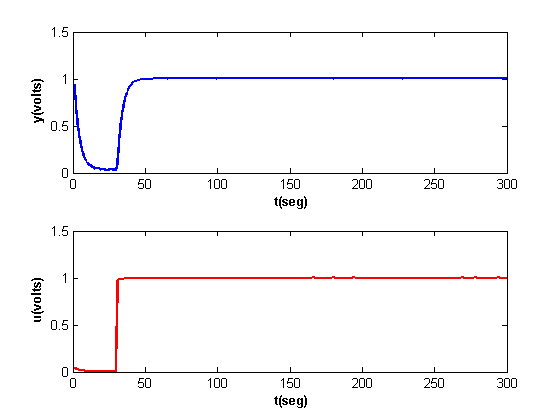
\includegraphics[width=0.45\textwidth]{./imagenes/data.png}
 	\caption{Data obtenida de la adquisici�n}
 	\label{fig:data}
\end{figure}

\begin{figure}[h!]
	\centering 
	\graphicspath{./imagenes/}
 	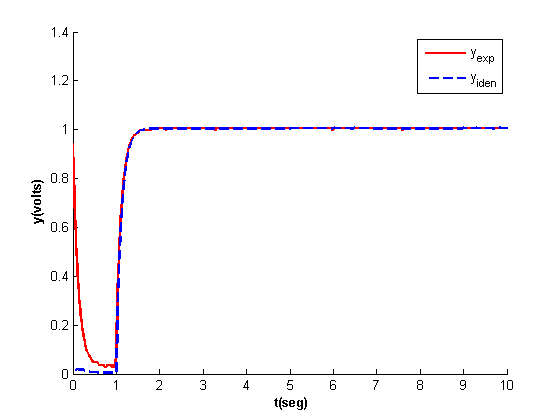
\includegraphics[width=0.45\textwidth]{./imagenes/identificacion_arx.png}
 	\caption{Identificaci�n ARX}
 	\label{fig:identificacion_arx}
\end{figure}

 
Se identifica el sistema usando la estructura param�trica ARX (ver Fig. ~\ref{fig:identificacion_arx}) usando una frecuencia de muestreo $f_{s}$ de $=30Hz$. Posteriormente, hallamos los controladores PI y exportamos los coeficientes obtenidos del controlador digital al directorio \textit{/data} para su procesamiento en labview. El c�digo generado es el siguiente:


\begin{lstlisting}
clear all; close all; clc
%% Programa para calcular el controlador
% -----------------
%% Cargando la DATA
% -----------------
dataLeida = load('../data/data_rc.lvm');
T=1/30; % Tiempo de Muestreo 
y1=dataLeida(:,4);
u1=dataLeida(:,6);

figure
subplot(211)
plot(y1,'b','LineWidth',2); 
xlabel('\bf t(seg)'); ylabel('\bf y(volts)');
subplot(212)
plot(u1,'r','LineWidth',2); 
xlabel('\bf t(seg)'); ylabel('\bf u(volts)');

% -------------------
%% Identificaci�n ARX
% -------------------
data=iddata(y1,u1,T);
th=arx(data,[1 1 1]);
present(th)
thc=d2c(th);
[num,den]=tfdata(thc);
Gp=tf(num,den)
gain = num{1}(2);
tau = 1/num{1}(2);

% -------------------
%% Polos de la planta 
% -------------------
sp=pole(Gp);
ip=abs(imag(sp));
rp=abs(real(sp));

% ------------------------------------------
%% Especificaciones de dise�o polos deseados
% ------------------------------------------
ts=1;
Mp=0.1;
zeta=-log(Mp)/sqrt((log(Mp))^2+pi^2);
wn=4.6/(zeta*ts);
s1=-zeta*wn+1j*wn*sqrt(1-zeta^2);
% Polo deseado
sd=s1;
id=abs(imag(sd));
rd=abs(real(sd));

% -------------------------------
%% Dise�o del control PI continuo
% -------------------------------
theta1=pi-atan(id/rd); 
theta2=atan((id-ip)/(rp-rd)); 
theta3=theta1+theta2+pi;   % condici�n de fase
theta3 = pi_to_pi(theta3); 

if abs(theta3)<pi/2
    zc = rd+id/tan(theta3);
else
    zc = rd-id/tan(theta3);
end
a = zc; % zero del controlador
% polo del controlador
sc = 0;

r1 = sd-sc; %polo
r2 = sd-sp; %polo
r3 = sd-zc; %zero

K = abs(r1)*abs(r2)/(gain*abs(r3));

% ---------------------------------------
%% Simulaci�n del Controlador PI continuo
% ---------------------------------------
Gc=tf(K*[1 a],[1 0])
% Funcion de transferencia en lazo cerrado H 
L=series(Gc,Gp);
H=L/(L+1)

figure; hold on;
t = 0:0.001:5;

u=ones(size(t));
yp=lsim(H,u,t);

plot(t,u,'r')
plot(t,yp, 'b', 'LineWidth',2)

xlabel('\bf t(seg)'); ylabel('\bf y(volts)');
legend('set point', 'y_{lazo cerrado}');

% ---------------------------------
%% Re-dise�o por tustin del Control 
%% en Tiempo Discreto
% ---------------------------------
T=tau/5;
[Nt,Dt] = tfdata(Gc,'v');
Nt = poly2sym(Nt,'s');
Dt = poly2sym(Dt,'s');
syms z
Gdt = Nt/Dt;
Gdt = subs(Gdt,{'s'},(2*(z-1))/(T*(z+1)));
Gdt = simplify(Gdt);
Gdt = vpa(Gdt,4); 
[NDt, DDt] = numden(Gdt);
NDt = sym2poly(NDt);
DDt = sym2poly(DDt);

% --------------------------------
%% FT del Controlador digital D(z)
% --------------------------------
GDt = tf(NDt,DDt,T)

% -------------------------------------
%% Coeficientes para lectura de LabVIEW
% -------------------------------------
[Np,Dp]=tfdata(Gp,'v');
planta = [Np Dp]; 
save '../data/coef_planta.lvm' planta -ascii -tabs
save '../data/num_controller.lvm' NDt -ascii -tabs
save '../data/den_controller.lvm' DDt -ascii -tabs
\end{lstlisting}


Finalmente podemos validar que las respuestas de los sistemas controlados por un controlador PI (ver Fig. ~\ref{fig:pi_sistema_controlado}) y PID (ver Fig. ~\ref{fig:pid_sistema_controlado}) en lazo cerrado cumplen con las condiciones de dise�o propuestas.





\begin{figure}[h!]
	\centering 
	\graphicspath{./imagenes/}
 	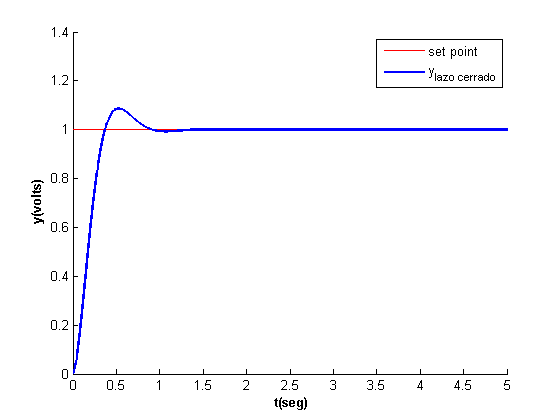
\includegraphics[width=0.45\textwidth]{./imagenes/pi_sistema_controlado.png}
 	\caption{Planta controlada usando un controlador PI}
 	\label{fig:pi_sistema_controlado}
\end{figure}

\begin{figure}[h!]
	\centering 
	\graphicspath{./imagenes/}
 	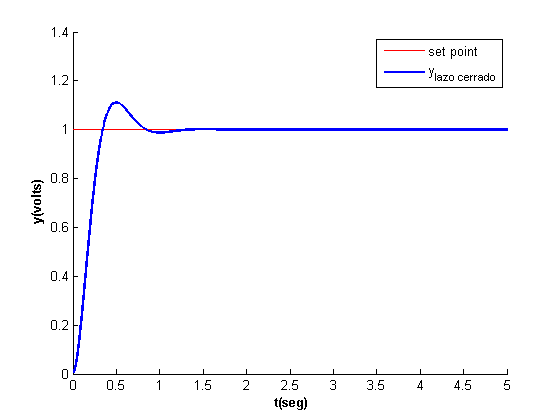
\includegraphics[width=0.45\textwidth]{./imagenes/pid_sistema_controlado.png}
 	\caption{Planta controlada usando un controlador PID}
 	\label{fig:pid_sistema_controlado}
\end{figure}




\section{CONCLUSIONES} %%%%%%%%%%%%%%%%%%%%%%%%%%%%%%%%%%%%%%%%%%%%%%%%%%%%%%%%%%%%%%%%%%%%%%%%%%%%%%%%%%%%%%%%%%%%%%%%%%%%%%%%%%%%%%%%%%%%%%%%%

\begin{itemize}
\item Notamos que comparando ambos controladores empleados (PI y PID), el sistema responde mejor frente al controlador PI ya que posee un menor sobre impulso ante el PID. (ver Fig. ~\ref{fig:compara_pi_pid})


\end{itemize}


\begin{figure}[h!]
	\centering 
	\graphicspath{./imagenes/}
 	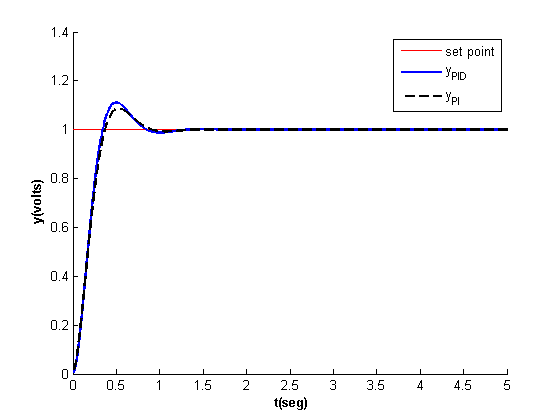
\includegraphics[width=0.45\textwidth]{./imagenes/compara_pi_pid.png}
 	\caption{Comparaci�n entre PI y PID}
 	\label{fig:compara_pi_pid}
\end{figure}


\bibliographystyle{IEEE} %%%%%%%%%%%%%%%%%%%%%%%%%%%%%%%%%%%%%%%%%%%%%%%%%%%%%%%%%%%%%%%%%%%%%%%%%%%%%%%%%%%%%%%%%%%%%%%%%%%%%%%%%%%%%%%%%

\nocite{*}
\bibliographystyle{IEEE}

\begin{thebibliography}{1}

\bibitem{}
Repositorios 
\newblock {\em https://github.com/oskargicast/ControladorPI}
\newblock 

\bibitem{}
Ing. Rodriguez Bustinza, Ricardo
\newblock {\em Dise�o del controlador discreto usando aproximador digital.}
\newblock 

\bibitem{}
Leonardo J. Mar�n, V�ctor M. Alfaro
\newblock {\em Sintonizaci�n de controladores por ubicaci�n de polos y ceros}
\newblock Departamento de Autom�tica, Escuela de Ingenier�a El�ctrica, Universidad de Costa Rica

\end{thebibliography}




\end{document}
